\documentclass{article}

% if you need to pass options to natbib, use, e.g.:
%     \PassOptionsToPackage{numbers, compress}{natbib}
% before loading milestone

% ready for submission
% \usepackage{milestone}

% to compile a preprint version, e.g., for submission to arXiv, add add the
% [preprint] option:
%     \usepackage[preprint]{milestone}

% to compile a camera-ready version, add the [final] option, e.g.:
     \usepackage[final]{milestone}
    
% to avoid loading the natbib package, add option nonatbib:
%     \usepackage[nonatbib]{milestone}

\usepackage[utf8]{inputenc} % allow utf-8 input
\usepackage[T1]{fontenc}    % use 8-bit T1 fonts
\usepackage{hyperref}       % hyperlinks
\usepackage{url}            % simple URL typesetting
\usepackage{booktabs}       % professional-quality tables
\usepackage{amsfonts}       % blackboard math symbols
\usepackage{nicefrac}       % compact symbols for 1/2, etc.
\usepackage{microtype}      % microtypography
\usepackage{graphicx}
\graphicspath{ {./images/} }
\title{Flappy Bird using Q-Learning}

% The \author macro works with any number of authors. There are two commands
% used to separate the names and addresses of multiple authors: \And and \AND.
%
% Using \And between authors leaves it to LaTeX to determine where to break the
% lines. Using \AND forces a line break at that point. So, if LaTeX puts 3 of 4
% authors names on the first line, and the last on the second line, try using
% \AND instead of \And before the third author name.

\author{%
  Jesse A. Pelzar\\
  Department of Electrical and Computer Engineering\\
  Binghamton University\\
  Binghamton, NY 13850\\
  \texttt{jpelzar1@binghamton.edu} \\
  \url{https://jessepelzar.github.io/Flappy_Bird_RL/}
  % examples of more authors
  % \And
  % Coauthor \\
  % Affiliation \\
  % Address \\
  % \texttt{email} \\
  % \AND
  % Coauthor \\
  % Affiliation \\
  % Address \\
  % \texttt{email} \\
  % \And
  % Coauthor \\
  % Affiliation \\
  % Address \\
  % \texttt{email} \\
  % \And
  % Coauthor \\
  % Affiliation \\e
  % Address \\
  % \texttt{email} \\
}

\begin{document}

\maketitle

\begin{abstract}
  The following is was developed in effort to implement an autonomous problem solving technique for minimal style mobile games. The game chosen for this project is the novel game Flappy Bird which requires the user to keep the player from coming in contact with moving obstacles by either jumping or not jumping within the game environment.  In order to do this, reinforcement learning methods were introduced, specifically Q-Learning in order to learn how to play the game and also includes editable values to test alternative configurations. 
\end{abstract}

\section{Introduction}

This project is based off of the well known mobile game Flappy Bird. With my strong background in web based technologies, I decided to recreate the game Flappy Bird within a web environment with the ability to not only play Flappy Bird, but the ability to have the the agent (the bird) learn how to avoid hitting the moving obstacles, floor or ceiling. The Reinforcement Learning component to this game was Q-Learning which allows the agent to learn through exploration and exploitation by optimizing the best action to take when in a given state. With a constantly changing environment, the agent must adapt to updated positioning of obstacles in order to avoid them. The importance of this project is to learn and adapt to a constantly changing environment while utilizing similarities such as comparing distances to achieve a different reward. The methods I incorporated are interesting and have the ability to be applied to other environments that may resemble a similar concept but consist of different states and actions.  

\section{Approach}

When considering the implementation of Reinforcement Learning, it's important to  determine what will make up the environment. this includes the actions, states, rewards and other variable such as a discount factor and exploration probability. Using Q-Learning, I was able to implement a model free learning approach that derives an optimal policy using time difference learning to constantly update the Q table values on each iteration. 

\subsection{Agent}

When a user is playing the flappy bird game, the bird's position is constrained to the x-axis, giving only the ability to move up and down on the y-axis. With this limited range, the actions are limited as well, in this case, jump or not jump. The standard jumping dynamics works by displacing the bird in the up direction by a jump multiplier value followed by a slow acceleration after the max height of the jump is reached. This gives it the realistic arching effect due to representing the rate of change induced by a gravity multiplier. 

When an average user of the flappy bird game plays the game, they must consider the time it takes for the bird to accelerate downwards in order to avoid collisions. This increases the difficulty for the user playing, giving the assumption that it will also be a challenge for the learning algorithm as well. When playing the game, the agent or bird must not come in contact with any surfaces such as the floor, ceiling or obstacle. 

Along with this standard jumping method, I also implemented a linear method that does not mimic physics but rather moves by a number of places in either the up direction or down direction. This method does not incorporate the same properties of physics that exists within the standard jump mode. When selected, input variables for the displacement up and displacement down can be set or adjusted. 

\subsection{Environment}
Obstacles in flappy bird spawn at a set time interval and consist of a top bar and a bottom bar positioned on the same x coordinate. The two obstacles share a gap between them that is set to a static value. The top and bottom bar heights are randomly selected by randomly choosing one bar and displacing the other bar by the set gap value. The vertical scale of the bars are also constrained between a minimum value and a maximum value, only allowing for a set range of random sizes to be selected for the bars. While the agent is fixed on the x axis, the top bar and bottom bar move in sync from right to left. Given a small gap compared to the entire height of the game area, the agent must maneuver its way between the opening, avoiding contact at all costs. In the case that the agent collides with an obstacle, the game will reset but the Q Table will not reset.


%Along with this standard jumping method, I also implemented a linear method that does not mimic physics but rather moves by a number of places in either the up direction or down direction.

\subsection{Choosing Actions}

In the game Flappy Bird, the bird is locked in x-space but has free range in the y-space. The actions capable by the bird are either jump or not jump. When the birds action is not jump, it will fall down to the ground, which loses the game. On the project website, you will have the ability to configure the type of jump that the agent can perform. The Standard jump mode is an arching jump that accelerates and decelerates, similar to the original game. The Linear jump mode has two variables that represent static jumping and falling velocities. In this project, the bird which represents the agent, must choose what states require a jump and which ones don't. 

\section{Components}

\subsection{Determining Environment States}

\begin{figure}[h]
    \centering
    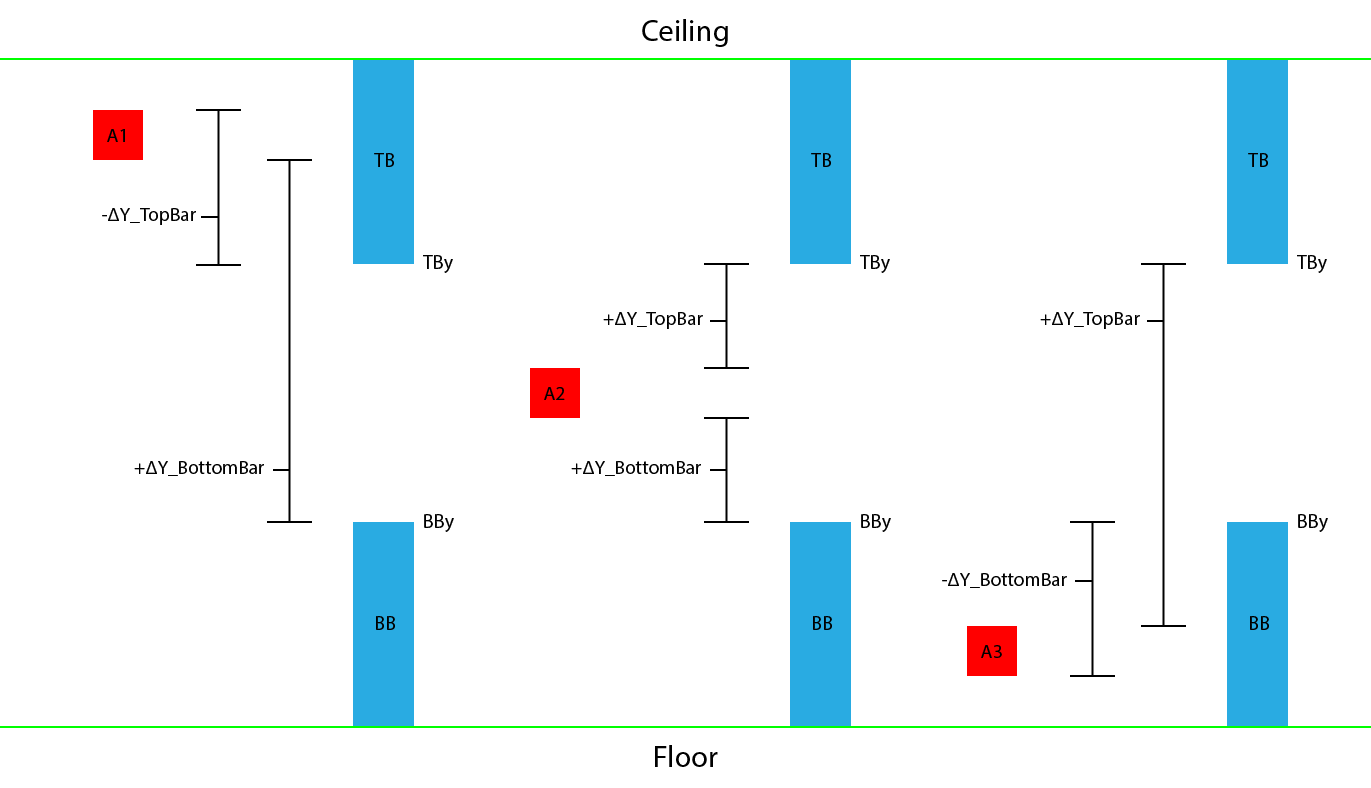
\includegraphics[width=0.75\textwidth]{figure0}
    \caption{Vertical Differencest}
    \label{fig:mesh1}
\end{figure}



In order for the agent to know its position in the environment, the agent must always be located in a state (s) which is a member of a discrete number of states in a set (S). States can be represented in a variety of ways including positioning in an environment, location relationships of obstacles, or even a combination of the two. In my development, I decided to represent the states by utilize the characteristics of the moving obstacles within the environment. These obstacles are referred to as the top bar, represented as TB and the bottom bar represented as BB, where TB is on the ceiling while BB is positioned directly below but on the floor. 



\subsection{Vertical Difference Between Agent Height and Obstacles}

When considering the states, rather than only using a single variable to represent the current state of the agent, the method I developed utilizes two variables. The first variable is derived from the vertical difference between top of the agent's height and the vertical position of TB's lowest part (TBy),  whereas the second variable is derived from the vertical difference between the bottom of the agent's height and the vertical position of BB's highest part (BBy).

Represented in figure 1, the agent is shown in three different positions, A1, A2, and A3. In position A1, the vertical difference between the top of the agent to the TBy scales negatively where as the vertical difference between the bottom of the agent to the BBy scales positively. With position A3 the vertical differences are the opposite of A1's with the vertical difference between the top of the agent to the TBy scales positively where as the vertical difference between the bottom of the agent to the BBy scales negatively. Last the position of A2 shows both of the vertical differences remaining positive. 


\begin{figure}[h!]
    \centering
    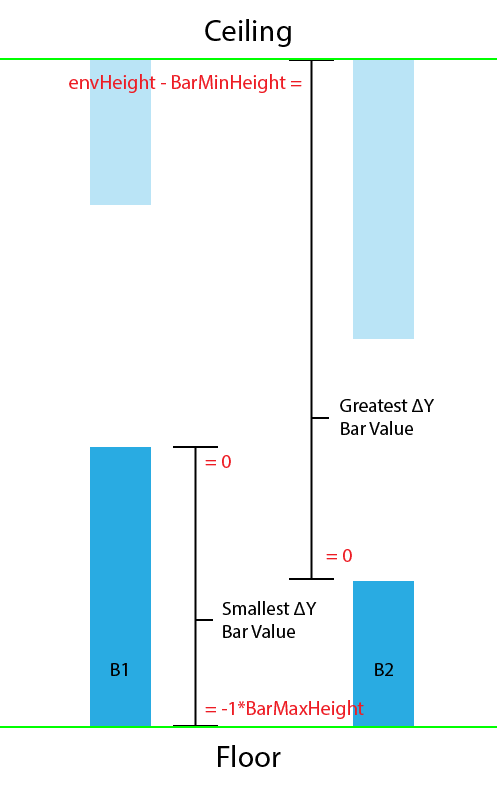
\includegraphics[width=0.5\textwidth]{figure2}
    \caption{Largest range of vertical distance values}
    \label{fig:mesh2}
\end{figure}

\subsection{Mapping to State Indexes}


In order to know the true range of vertical difference from the smallest negative value to the largest positive value, it's important to know the maximum height of an obstacle as well as the minimum height. This tells us that the lowest value the state can be is the length of the tallest obstacle multiplied by negative 1 and that the greatest value the state can be is the height of the shortest obstacle subtracted from the height of the environment, in this case the game canvas. This is visually represented in figure 2. Gathering the values from the vertical differences for the purpose of representing states means that when indexing the Q table, all of the indexes must be positive. When running, these values are stored as class variables that are passed as arguments to a function that maps them to positive integers. The mapping of the values also grants the ability to choose the range from zero to the number of desired states represented in figure 3. This variable is modifiable on the project webpage. 

\begin{figure}[h!]
    \centering
    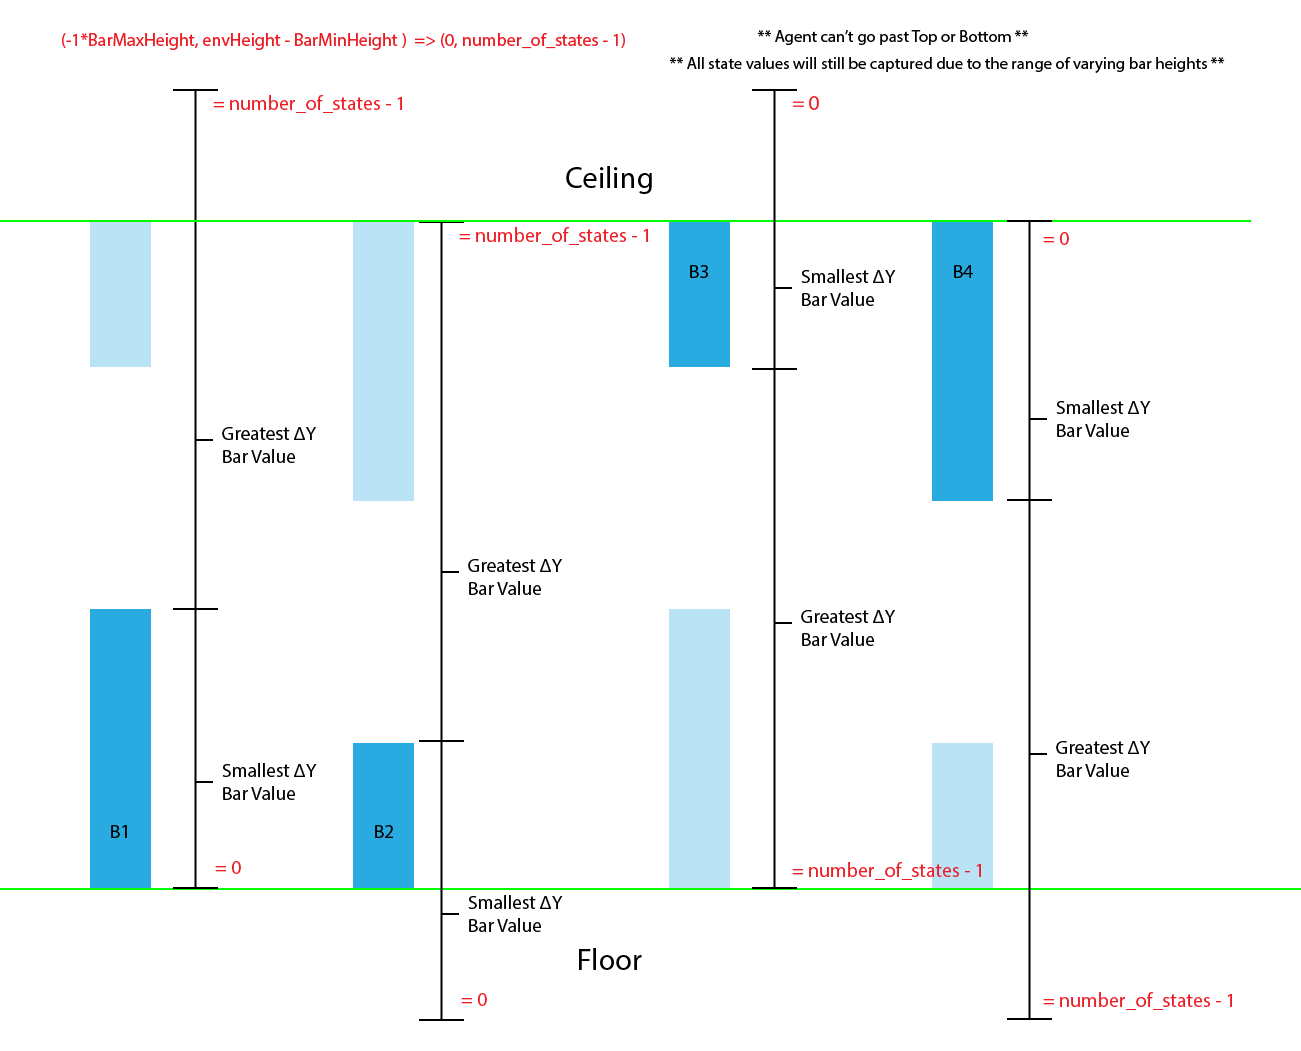
\includegraphics[width=1\textwidth]{figure3}
    \caption{Largest range of vertical distance values mapped}
    \label{fig:mesh2}
\end{figure}

\subsection{Rewards}

\begin{figure}[h!]
    \centering
    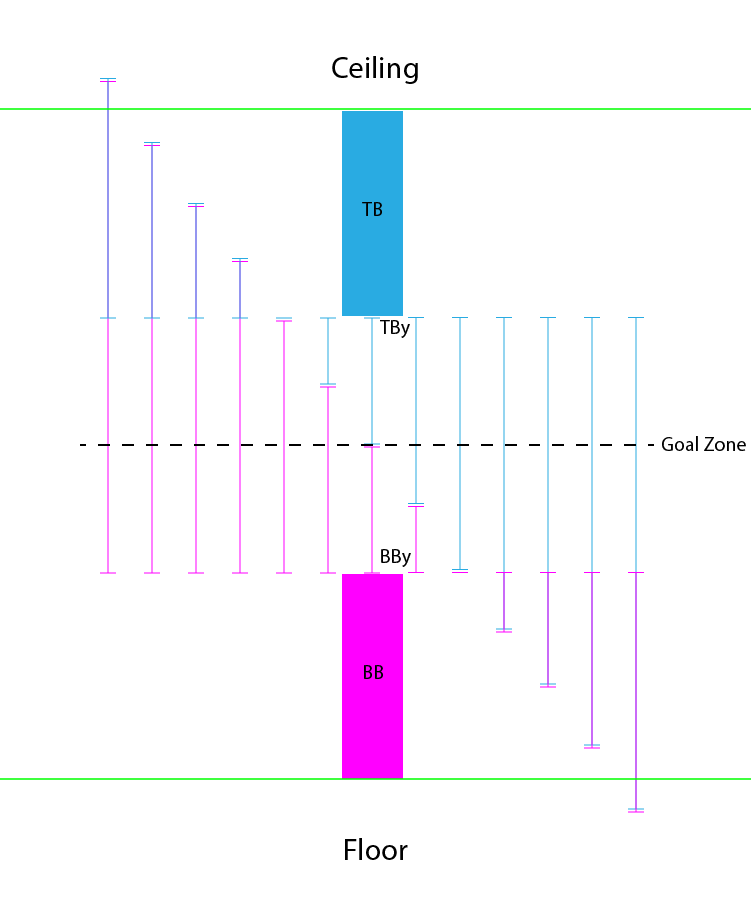
\includegraphics[width=1\textwidth]{figure4}
    \caption{Example of reward zones}
    \label{fig:mesh2}
\end{figure}

Rewards are necessary for telling the agent if a chosen action for a set of states is the best action to take. Utilizing the vertical difference algorithm to do this reduces the need for additional processes and is overall more efficient. Because the objective of the agent is to make it through the gap between the obstacles, veering away from this goal zone must issue a penalty or negative reward. The method I came up with is shown in figure 4 and mathematically represented in the equation below. Taking the absolute value of the difference between TBy and BBy and raising it to a power of some value will exponentially increase as the difference becomes larger. When multiplied by negative one, the reward value decreases exponentially by the power it was raised too. With an exponentially decreasing reward, the further the agent moves from the goal zone, the larger the penalty will be.
\begin{equation}
Reward = (|TBy-BBy|^{x}) * -1
\end{equation}

\section{Results}

\subsection{Experiental Results}
When designing the controls for the Flappy Bird Q-Learning website, I considered the ability to change values such as the number of states, number of episodes, number of iterations, gamma for the reward discounts, epsilon for the exploration rate, and the reward exponent. In addition, I also included various running speeds and two jump modes. With these additions to the website I conducted tests for these inputs allowing a max score of either 100 or 1000. 

Beginning with the reward discount, gamma, viewing figure 5 shows the scores that were received from when gamma was set to 0.9 to when it was set to 0.1. As the gamma value approached 0.5, the max score of 100 with 100 percent efficiency was achieved. With this realization, I was able to acknowledge that the agent will be searching for immediate rewards equally as much as future rewards because there does not exist a final goal state that will terminate the game but instead exists the need to continuously try to maintain itself within a state region which can almost be considered a goal state. 

Next I tested my exploration value epsilon, which was compared to a random number generated each iteration. This works by testing when a random number becomes less than epsilon, rather than comparing the maximum ranked action for a given state, a random action is selected. This gives the agent a chance to explore other possibilities that it may not consider when exploiting the existing state's actions. For the tests, I tested epsilon values ranging from 0.1 to 0.9 in increments of 0.1.The results shown in figure 6 show that the highest success was achieved at lower epsilon values rather than high ones.

While developing the algorithm, I had to consider the amount of states the agent can potentially be in. To achieve the best results, I ran tests for different amounts of states consisting of all odd values between 1 and 17. Before running the tests, my theory of the results was that I believed the smaller number of states meant that less computation was required in order to reach an optimal policy. This theory served to be correct, giving scores surpassing the max amount of 1000 points for state amounts 3, 5, 7, and 10. This data is represented in figure 7. 

Iterations play an important role to the learning process due to the fact that each update of the environment and the agent is one iteration. For this test, I reduced the amount of episodes which are responsible for grouping the amount of iterations for faster policy development. I then ran the learning process and recorded the results for iteration counts from 1 to 50000. Viewing figure 8, It's obvious that the greater amount of iterations showed the best results when running the developed policy. 

From the data I collected through the testing process, I was able to find the 
\section{Conclusion}
With technology advancing in the direction of automation and artificial intelligence, it has become a greater desire for me to learn the many aspects involved such as reinforcement learning. This project helped me obtain a better understanding on how Q-Learning functions and how versatile it can be when incorporated within other environments. Some of the unresolved issues and inconsistencies I ran into come from the agent not being exposed to every state. To solve this in the future, I would like to include other conditions which force the agent to test all states but in a deterministic manner rather than being random. This way, the agent can deterministically explore states that have been missed which can patch any holes leading to more certain decision making. This class and especially this project has motivated me to explore new areas of reinforcement learning and its applications to new ideas and environments. What I learned is that with each algorithm or combination of algorithms, any environment consists of states, agents, and actions can be controlled, learned or ran by a basic or complex artificial intelligence.

\begin{figure}[h!]
    \centering
    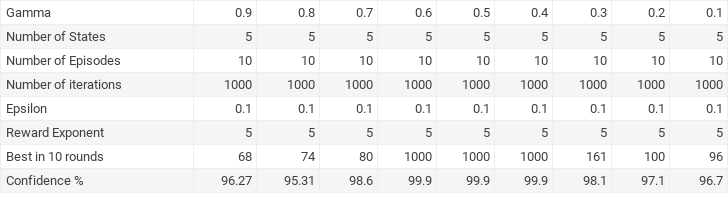
\includegraphics[width=1\textwidth]{figure5}
    \caption{Gamma Range Values}
    \label{fig:mesh2}
\end{figure}

\begin{figure}[h!]
    \centering
    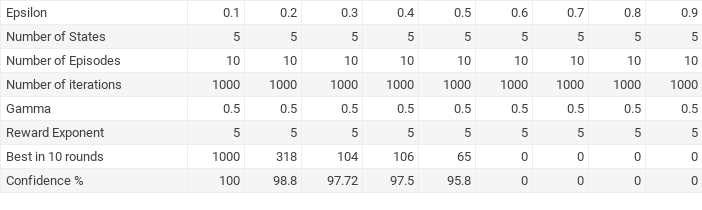
\includegraphics[width=1\textwidth]{figure6}
    \caption{Gamma Range Values}
    \label{fig:mesh2}
\end{figure}

\begin{figure}[h!]
    \centering
    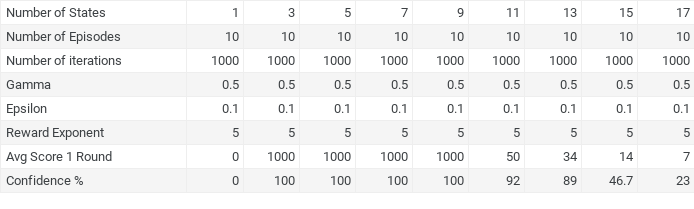
\includegraphics[width=1\textwidth]{figure7}
    \caption{Gamma Range Values}
    \label{fig:mesh2}
\end{figure}

\begin{figure}[h!]
    \centering
    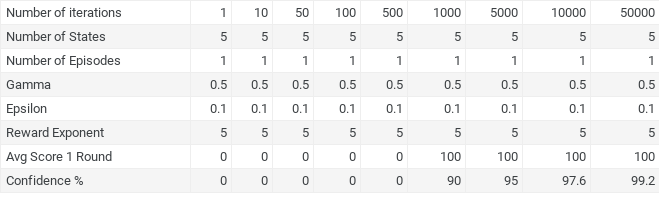
\includegraphics[width=1\textwidth]{figure8}
    \caption{Gamma Range Values}
    \label{fig:mesh2}
\end{figure}



\section*{References}

[1] Choudhary, Ankit. “Deep Q-Learning: An Introduction To Deep Reinforcement Learning.” Analytics Vidhya, 27 Apr. 2020, www.analyticsvidhya.com/blog/2019/04/introduction-deep-q-learning-python/.


\end{document}